\documentclass{article}
\usepackage[margin=0.5in]{geometry}
\usepackage{amsmath}
\usepackage{float}
\usepackage{tikz}
\usetikzlibrary{patterns}
\usepackage{graphicx} % Required for inserting images

\title{Numerical Solution of ODEs using Trapezoidal Rule and Newton-Raphson}
\author{Himanshu Jindal, Shubham Vishwakarma, Kaustubh Dandegaonkar}
\date{}

\begin{document}
\maketitle

\section*{Problem Statement}
Solving System of Differential Equations

Define the vector of dependent variables $\mathbf{Y}$ and the vector of functions $\mathbf{F}(x, \mathbf{Y})$:

\begin{align}
    \mathbf{Y} &= \begin{bmatrix} y_{1} \\ y_{2} \\ y_{3} \end{bmatrix} \\
    \mathbf{F}(x, \mathbf{Y}) &= \begin{bmatrix} f_1(x, \mathbf{Y}) \\ f_2(x, \mathbf{Y}) \\ f_3(x, \mathbf{Y}) \end{bmatrix}
\end{align}


The system of differential equations can be expressed as:

\begin{align}
    \textbf{Y}' &= \mathbf{F}(x, \mathbf{Y})
\end{align}

\section*{Numerical Solution Using Trapezoidal Rule}

To numerically solve this system of differential equations, we employ the Trapezoidal Rule for time discretization. The Trapezoidal Rule is a numerical integration method that can be adapted for solving differential equations.

Let $h$ be the step size and $x_i = x_0 + i \cdot h$. The Trapezoidal Rule updates the solution at each step as follows:

\begin{align}
    \mathbf{Y}^{(i+1)} &= \mathbf{Y}^{(i)} + \frac{h}{2} \left[ \mathbf{F}(x_i, \mathbf{Y}^{(i)}) + \mathbf{F}(x_{i+1}, \mathbf{Y}^{(i+1)}) \right]
\end{align}

Here, $\mathbf{Y}^{(i)}$ represents the solution at the $i$-th step, and $\mathbf{F}(x, \mathbf{Y})$ is the vector function defining the differential equations.

\section*{Theoretical Error Analysis}

The error analysis involves understanding the difference between the numerical solution and the exact solution. Let's consider the local truncation error and the global error.

\subsection*{Local Truncation Error}

The local truncation error at each time step is the error introduced by a single application of the numerical method. 
$$
T_n = \frac{y(x_{n+1}) - y(x_n)}{h} - \frac{1}{2} [ f(x_n, y_n) + f(x_{n+1}, y_{n+1}))
$$
For the Trapezoidal Rule, the local truncation error is proportional to the third derivative of the solution and the square of the step size $h$. The local truncation error for each component of the vector $\mathbf{Y}$ can be expressed as:

\begin{align}
    \text{T}_1 &= \frac{h^2}{12} y_{1}'''(t) + \mathcal{O}(h^3), \\
    \text{T}_2 &= \frac{h^2}{12} y_{2}'''(t) + \mathcal{O}(h^3), \\
    \text{T}_3 &= \frac{h^2}{12} y_{3}'''(t) + \mathcal{O}(h^3).
\end{align}

Here, $\text{T}_1, \text{T}_2,$ and $\text{T}_3$ represent the local truncation error for $y_{1}, y_{2},$ and $y_{3}$, respectively.

\subsection*{Global Error}

The global error is the cumulative error over the entire solution interval. It is influenced by the local truncation error at each step and the total number of steps taken. The global error is typically proportional to the step size $h$ and is given by:

\begin{align}
    \text{Global Error} &= \mathcal{O}(h^2).
\end{align}

This indicates that by reducing the step size, the global error can be effectively decreased.

\section*{Newton-Raphson Method for Iterative Solution}

The numerical solution using the Trapezoidal Rule is implicit and requires an iterative solution. We utilize the Newton-Raphson method for solving the nonlinear equation:

\begin{align}
    \mathbf{F}(\mathbf{Y}_{n+1}) &= \mathbf{Y}_{n} + \frac{h}{2}[\mathbf{F}(x_{n}, \mathbf{Y}_{n}) + \mathbf{F}(x_{n+1}, \mathbf{Y}_{n+1})] - \mathbf{Y}_{n+1}
\end{align}

The Newton-Raphson iteration is employed to find $\mathbf{Y}_{n+1}$ such that $\mathbf{F}(\mathbf{Y}_{n+1}) = \mathbf{0}$. The iterative process is governed by:

\begin{align}
    \mathbf{Y}_{k+1} &= \mathbf{Y}_{k} - [\mathbf{J_F}(\mathbf{Y}_{k})]^{-1} \mathbf{F}(\mathbf{Y}_{k})
\end{align}

where $\mathbf{J_F}(\mathbf{Y}_{k})$ is the Jacobian matrix of $\mathbf{F}$ evaluated at $\mathbf{Y}_{k}$.


\section*{Problem Statement 1}
Solving System of Differential Equations:

\begin{align*}
    y_1' &= -2y_1 + y_2 - 2y_3\\
    y_2' &= y_1 - 2y_2 + 2y_3 \\
    y_3' &= 3y_1 - 3y_2 + 5y_3
\end{align*}

Initial conditions:
\begin{align*}
    y_1(0) &= -2 \\
    y_2(0) &= 2 \\
    y_3(0) &= 4
\end{align*}
\subsection*{Explanation of the Code and Graphs}

The provided Python code implements the numerical solution of the given system of differential equations using the Trapezoidal Rule and the Newton-Raphson method. The functions defined in the code correspond to the system of differential equations, and the main solver uses newton raphson for implicit calculations.

The graphs below depict the numerical solutions (solid lines) obtained by the Trapezoidal Rule and Newton-Raphson method. The exact solutions (dashed lines) are also plotted for comparison. The solutions are calculated over the interval $[0, 1]$ with a step size of $0.0001$.
\begin{figure}[H]
    \centering
    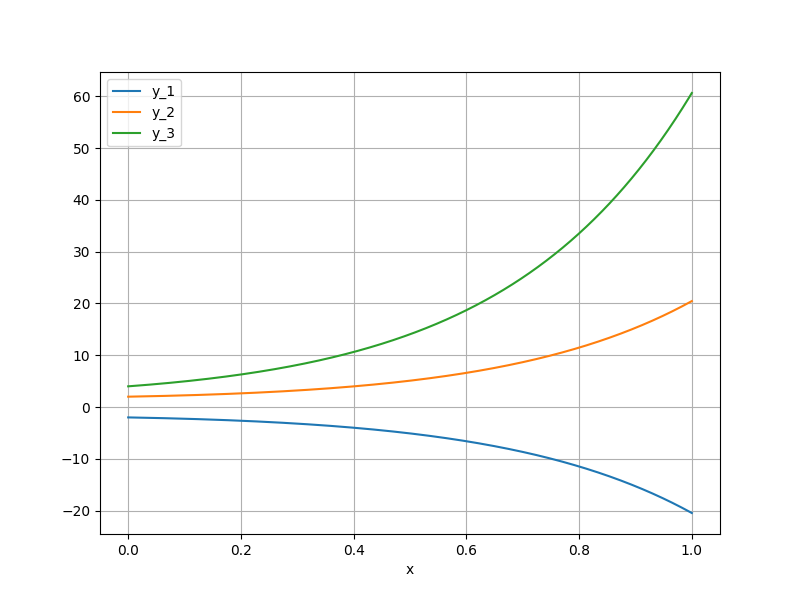
\includegraphics[width = 13cm]{save.png}
    \caption{Caption}
    \label{fig:solutions}
\end{figure}
The figure \ref{fig:solutions} illustrates the accuracy of the numerical method by comparing the computed solutions with the exact solutions. The code provides insights into the implementation of numerical methods for solving differential equations.

\section*{Problem Statement 2}
Consider an electrical circuit consisting of an inductor (L), a resistor (R), and a capacitor (C) described by the following second-order linear differential equation:

\[
L\frac{d^2Q}{dt^2} + R\frac{dQ}{dt} + \frac{1}{C}Q = V(t)
\]

where:
\begin{itemize}
  \item \( Q(t) \) is the charge in the circuit at time \( t \),
  \item \( L = 1 \, \text{H} \) is the inductance,
  \item \( R = 40 \, \Omega \) is the resistance,
  \item \( C = \frac{1}{4000} \, \text{F} \) is the capacitance,
  \item \( V(t) = 24 \, \text{V} \) is the applied voltage.
\end{itemize}

The initial conditions are \( Q(0) = 0 \) and \( \frac{dQ}{dt}(0) = 0 \).

This is similar to Solving System of Differential Equations:

\begin{align*}
    \frac{dI}{dt} &= -40I - 4000Q + 24 \\
    \frac{dQ}{dt} &= I
\end{align*}

Initial conditions:
\begin{align*}
    Q(0) &= Q_0 = 0 \\
    I(0) &= I_0 = 0
\end{align*}
\subsection*{Graphs obtained by the Trapezoid Rule}
h = $5 \times 10^{-5}$
\begin{figure}[H]
    \centering
    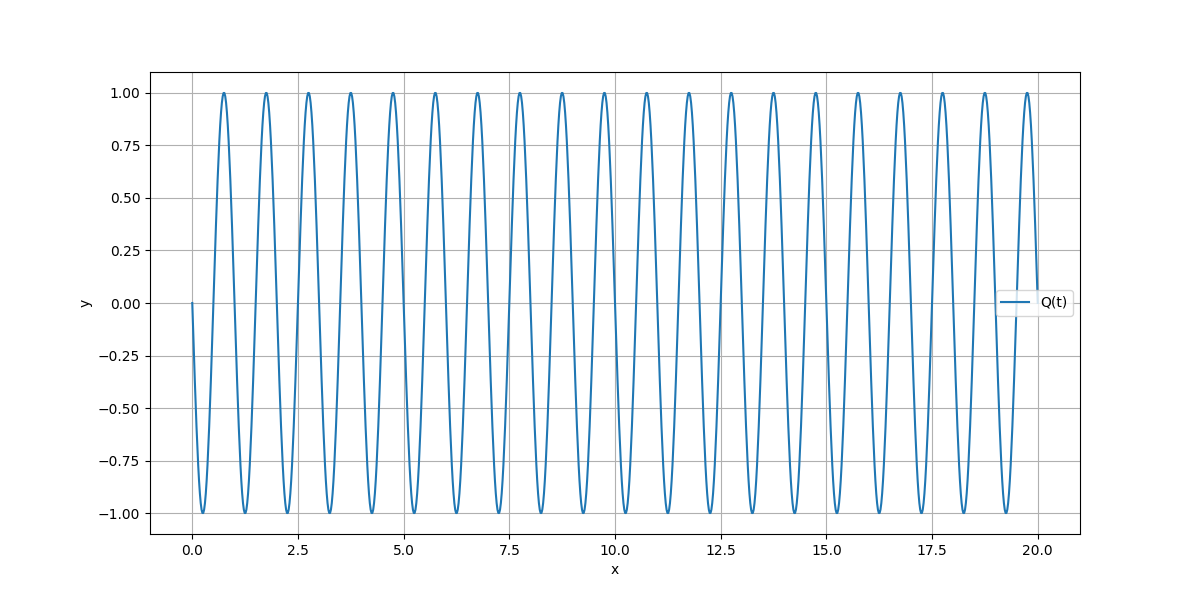
\includegraphics[width = 13cm]{save_0.png}
    \caption{Charge}
    \label{fig:Charge}
\end{figure}

\begin{figure}[H]
    \centering
    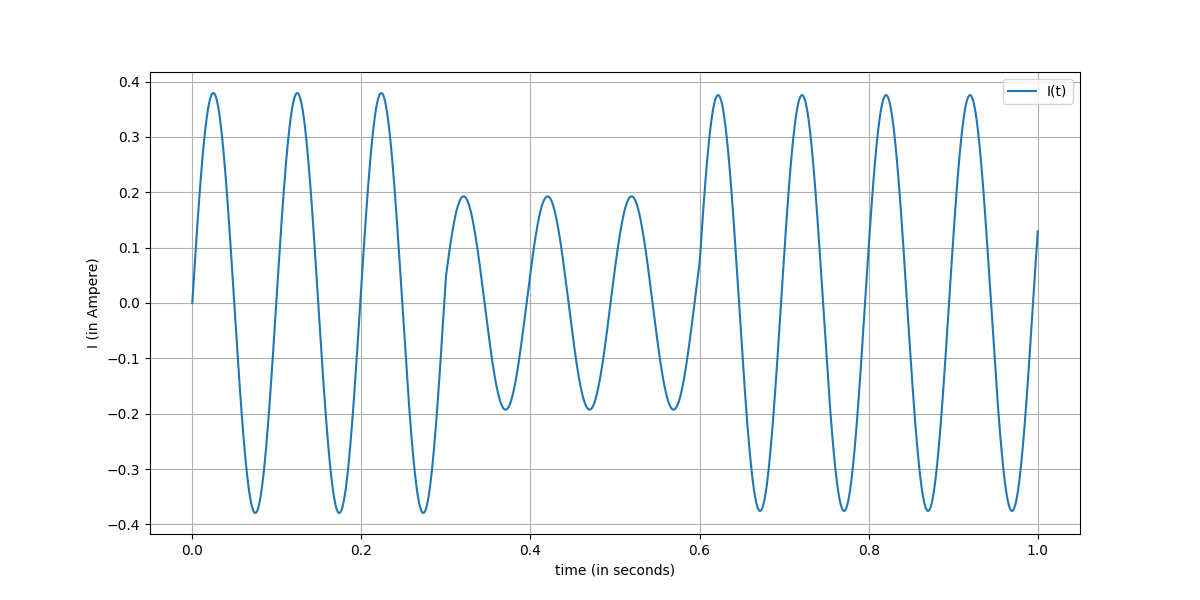
\includegraphics[width = 13cm]{save_1.png}
    \caption{Current}
    \label{fig:Current}
\end{figure}

\subsection*{Actual Graphs}

\begin{figure}[H]
    \centering
    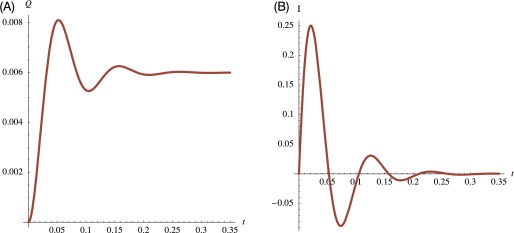
\includegraphics[width = 13cm]{Expected.jpg}      
    \caption{Actual Graphs}
    \label{fig:Actual Graphs}
\end{figure}

\section*{Solving 2nd Order Linear Differential equation}
\begin{align}
    a\cdot\frac{d^2x}{dt^2}+b\cdot\frac{dx}{dt}+c\cdot x &= f(t) \label{eq:2d}\\
    a\cdot\frac{d^2x}{dt^2}+b\cdot\frac{dx}{dt}+c\cdot x &= 0 \label{eq:2dhomo}
\end{align}

\noindent Here $x(t)$ is a dependent on $t$\\\\
Consider the solution space of (\ref{eq:2d}).
Let $x_1(t)$ and $x_2(t)$ be solutions of (\ref{eq:2d}). Then $x_1(t) - x_2(t)$ is a solution of (\ref{eq:2dhomo})\\
So once we find a particular solution $x_p(t)$ of (\ref{eq:2d}). The other solutions are of the form $x_p(t) + x_g(t)$ for some $x_g(t)$ which is solution for (\ref{eq:2dhomo})\\\\
So let us first consider the solutions of (\ref{eq:2dhomo})\\
Note : The solutions of (\ref{eq:2dhomo}) form a vector space with dim = 2.\\
The basis vectors (solutions) depends of the values of a,b,c.\\
We can look for solutions of form $x(t) = e^{kt}$.\\
Now,\\
\begin{align}
    (a\cdot k^2 +b\cdot k+c)\cdot e^{kt} &= 0 \label{eq:quad}
\end{align}
Now finding the roots of below quadratic in $k$ we get\\
\begin{align*}
    (a\cdot k^2 +b\cdot k+c) = 0
\end{align*}
Three cases\\
\begin{enumerate}
    \item Both roots are real and distinct\\
    Let $\alpha$ and $\beta$ be solutions of above then $e^{\alpha t}$ and $e^{\beta t}$ are solution of (\ref{eq:2dhomo})\\
    \item Both roots are real and equal\\
    One solution we get is $e^{rt}$ where r is root of (\ref{eq:quad})\\
    The other solution is $t\cdot e^{rt}$ which can be verified\\
    \item If the roots are not real\\
    Let the roots be ($\alpha \pm i \cdot \beta$)\\
    Then the two solutions are $e^{\alpha t} \cdot sin(\beta t)$ and $e^{\alpha t} \cdot cos(\beta t)$\\
\end{enumerate}

\noindent Now we have to solve for $x_p(t)$ also called particular solution of (\ref{eq:2d})\\
We will look at few cases of $f(t)$\\
\begin{enumerate}
    \item $f(t)$ is constant\\
    Let $f(t) = d$\\
    \begin{itemize}
        \item If $c \neq 0$\\
        $x_p(t) = \frac{d}{c}$\\
        \item If c = 0\\
        $x_p(t) = \frac{d}{b}\cdot x$
    \end{itemize}

    \item $f(t) = A\cdot sin(\omega t) + B\cdot cos(\omega t)$\\
    \begin{itemize}
        \item $b = 0$ and $c = w^2$\\\\
        $x_p(t) = -\frac{A t cos(\omega t)}{2\omega} + \frac{B t sin(\omega t)}{2\omega}$\\
        \item $b \neq 0$ or $c \neq w^2$\\
        $$\alpha = \frac{
            \begin{vmatrix}
        A & -b\omega \\
        B & c-\omega^{2} \\
        \end{vmatrix}}{
            \begin{vmatrix}
            c-\omega^2 & -b\omega \\
            b\omega & c-\omega^2 \\
             \end{vmatrix}
        }, \quad
        \beta = \frac{
            \begin{vmatrix}
            c-\omega^2 & A \\
            b\omega & B \\
            \end{vmatrix}
        }{\begin{vmatrix}
            c-\omega^2 & -b\omega \\
            b\omega & c-\omega^2 \\
             \end{vmatrix}
        }$$\\

        $x_p = \alpha \cdot sin(\omega t) + \beta \cdot cos(\omega t)$
        
    \end{itemize}
    
    Now we will try to solve the below equation\\
    with $a = b = 1, A = -1, B = 0, w = 2\pi$\\
    \begin{align}
        \frac{d^2x}{dt^2}+\frac{dx}{dt}+c\cdot x = -sin(2 \pi t), \quad \label{eq:test_ode}
        x(0) = 0,\quad x'(0) = 0
    \end{align}
    $$\alpha = \frac{
        \begin{vmatrix}
    -1 & -2\pi \\
    0 & 1 - 4\pi^2 \\
    \end{vmatrix}}{
        \begin{vmatrix}
        1 - 4\pi^2 & -2\pi \\
        2\pi & 1-4\pi^2 \\
         \end{vmatrix}
    }, \quad \beta = \frac{
        \begin{vmatrix}
        1-4\pi^2 & -1 \\
        2\pi & 0 \\
        \end{vmatrix}
    }
    {
        \begin{vmatrix}
        1 - 4\pi^2 & -2\pi \\
        2\pi & 1-4\pi^2 \\
         \end{vmatrix}
    }$$
    $$\alpha = \frac{4\pi^2-1}{4\pi^2 + (1-4\pi)^2}, \quad \beta = \frac{-2\pi}{4\pi^2 + (1-4\pi)^2}$$\\
    $$\alpha = 0.025313631977177762, \quad \beta = -0.004133492238317597$$
    $x_p(t) = \alpha \cdot sin(2\pi t) + \beta \cdot cos(2\pi t)$\\
    $x_g(t) = e^{-t/2} \cdot (c_1 \cdot sin(\sqrt{3}t/2) + c_2 \cdot cos(\sqrt{3}t/2))$
    
    Solution of (\ref{eq:test_ode})\\\\
    $x(t) = x_p(t) + x_g(t)$\\\\
    $x(t) = \alpha \cdot sin(2\pi t) + \beta \cdot cos(2\pi t) + e^{-t/2} \cdot (c_1 \cdot sin(\sqrt{3}t/2) + c_2 \cdot cos(\sqrt{3}t/2))$
    \subsection*{Analysis}
    Here as we can see in $x_g$ is of the form  $e^{-t/2} \cdot (sinusoids).$ So as time increases the amplitude of the sinusoids decreases.\\
    So as t increases the solution $x(t)$ approaches $x_p(t)$\\


    Let us anyway solve for $c_1$ and $c_2$ satisfying the initial conditions\\\\
    $x(0) = \alpha \cdot sin(2\pi \cdot 0) + \beta \cdot cos(2\pi \cdot 0) + e^{-0/2} \cdot (c_1 \cdot sin(\sqrt{3} \cdot 0) + c_2 \cdot cos(\sqrt{3} \cdot 0))$\\
    $x(0) = \alpha \cdot sin(0) + \beta \cdot cos(0) + c_2$\\
    $x(0) = \beta + c_2 = 0$\\
    $c_2 = -\beta$\\\\
    $x'(t) = 2\pi \cdot \alpha \cdot cos(2\pi t) - 2\pi \cdot \beta \cdot sin(2\pi t) - \frac{1}{2} \cdot e^{-t/2} \cdot (c_1 \cdot sin(\sqrt{3}t/2) + c_2 \cdot cos(\sqrt{3}t/2)) + e^{-t/2} \cdot (c_1 \cdot \frac{\sqrt{3}}{2} \cdot cos(\sqrt{3}t/2) - c_2 \cdot \frac{\sqrt{3}}{2} \cdot sin(\sqrt{3}t/2))$\\
    $x'(0) = 2\pi \cdot \alpha - \frac{1}{2} \cdot c_2 + \frac{\sqrt{3}}{2} \cdot c_1$\\
    $c_1 = -\frac{4}{\sqrt{3}}\pi \cdot \alpha - \frac{\beta}{\sqrt{3}}$\\
    Calculating numerical value of $c_1$ and $c_2$\\
    $c_1 = -0.18126892549017007$\\
    $c_2 = 0.004133492238317597$\\
\end{enumerate}

\section{Solving for Square wave function}

The objective is to solve the differential equation
\[ ax'' + bx' + cx = f(t) \]
where \( f(t) \) is a square wave function defined as follows:

\[
f(t) =
\begin{cases}
1 & \text{if } 0 \leq t < p \\
0 & \text{if } p \leq t < 1
\end{cases}
\]

This function is periodic with period \( T = 1 \).

\begin{figure}[h]
\centering
\begin{tikzpicture}
% Axis
\draw[->] (-0.5,0) -- (6,0) node[right] {\( t \)};
\draw[->] (0,-0.5) -- (0,1.5) node[above] {\( f(t) \)};
% Function
\draw[thick] (0,1) -- (2,1) -- (2,0) -- (4,0) -- (4,1) -- (6,1);
% Period markings
\draw[dashed] (2,0) -- (2,-0.2) node[below] {\( p \)};
\draw[dashed] (4,0) -- (4,-0.2) node[below] {1};
\end{tikzpicture}
\caption{Square wave function \( f(t) \) with period \( T=1 \) and amplitude \( A=1 \)}
\label{fig:square_wave}
\end{figure}

We have the following initial conditions for the differential equation:
\[ x(0) = 0 \]
\[ x'(0) = 0 \]

We convert the square wave to its Fourier transform, which is equal to:

\[
p + \sum_{n=1}^{\infty} \left( A_n \cos(2\pi n t) + B_n \sin(2\pi n t) \right)
\]

where \( A_n \) and \( B_n \) are the Fourier coefficients, and \( p \) is the average value of the function.
\(A_n\) and \(B_n\) are given by the following equations:

\[A_n = \frac{2}{T} \int_{0}^{T} f(t) \cos(2\pi n t) \, dt = \frac{sin(2 \pi n p)}{\pi n}\]
\[B_n = \frac{2}{T} \int_{0}^{T} f(t) \sin(2\pi n t) \, dt = \frac{1 - \cos(2 \pi n p)}{\pi n}= \frac{2 sin^2(\pi n p)}{\pi n}\]

We approximate this by the truncated Fourier series:

\[
f_N(t) = p + \sum_{n=1}^{N} \left( A_n \cos(2\pi n t) + B_n \sin(2\pi n t) \right)
\]

where \( N \) is the number of terms used in the approximation.

The equation to solve is:

\[
ax'' + bx' + cx = f_N(t)
\]

with initial conditions:

\[
x_N(0) = 0, \quad x'_N(0) = 0
\]

where \( f_N(t) \) is the truncated Fourier series of \( f(t) \) with \( N \) terms,
and \( x_N(t) \) is the solution to the differential equation with \( f_N(t) \).

We have the equation:
\begin{equation}
x_N(t) = x_{N,\text{particular}}(t) + x_{N,\text{homogeneous}}(t)
\end{equation}

Now, let's consider the homogeneous solution \(x_{N,\text{homogeneous}}(t)\). 

The homogeneous equation is given by:
\[
ax'' + bx' + cx = 0
\]

Consider the solution space of this equation. Let \(x_1(t)\) and \(x_2(t)\) be solutions. Then \(x_1(t) - x_2(t)\) is a solution of the homogeneous equation.

To find solutions of the homogeneous equation, we consider the characteristic equation:
\[
a k^2 + b k + c = 0
\]

Depending on the roots of this equation, the solutions of the homogeneous equation vary:
\begin{enumerate}
    \item If both roots are real and distinct (\( \alpha \) and \( \beta \)), then \( e^{\alpha t} \) and \( e^{\beta t} \) are solutions.
    \item If both roots are real and equal (\( r \)), then \( e^{rt} \) and \( t e^{rt} \) are solutions.
    \item If the roots are complex (\( \alpha \pm i \beta \)), then \( e^{\alpha t} \sin(\beta t) \) and \( e^{\alpha t} \cos(\beta t) \) are solutions.
\end{enumerate}

These solutions form a vector space with dimension 2, and the basis vectors (solutions) depend on the values of \(a\), \(b\), and \(c\).

Now, we have to solve for \(x_{N,\text{particular}}(t)\), also called the particular solution of \(x_N\).

In the context of our problem, the particular solution \( x_{N,\text{particular}} \) is expressed as the sum of the constant term \( \tilde{x}_0 \) and a series of terms \( \tilde{x}_n \) for \( n = 1, 2, \ldots, N \), representing the contribution of each Fourier component:
\[ x_{N,\text{particular}} = \tilde{x}_0 + \sum_{n=1}^{N} \tilde{x}_n \]

where \( \widetilde{x}_{N,\text{particular}}(t) \) is the particular solution of \(ax'' + bx' + cx = f_N(t)\), \( \widetilde{x}_0 \) is the particular solution of \(ax''+bx'+cx = p\), and \( \widetilde{x}_n \) is the particular solution of \(ax''+bx'+cx = A_n \cos(2 \pi n t) + B_n \sin(2 \pi n t)\).

Calculating the particular solution of \(ax''+bx'+cx = p\), we have the following cases:
\begin{itemize}
    \item If \(c \neq 0\), then
    \[
        \widetilde{x}
        _{0}(t) = \frac{p}{c}
    \]
    \item If \(c = 0\), then
    \[
        \widetilde{x}
        _{0}(t) = \frac{p}{b} \cdot t
    \]
\end{itemize}

\end{document}